% what is offloaded to proxy and we achieve lower overhead? Check presentation
% tool resolution
%What should I conclude on this topic? That indeed this SDK is useful for iot transacting with the network and how important it is to have their own unique identities? Assignment of identities are out of scope but we could describe how it can be done with secure enclaves.
%Experiments done with only 1 transaction in a setup of one endorsers. More endorsers mean more transaction proposal responses and more traffic as well. 
% measure voltage of rpi with the usb: Nothing notable from 0.29A idling to 0.37A, I would say averaging around 0.35A so a 0.05A while transacting. 50mA
% Could add bar graphs instead of tables or could add percentages on tables.
\chapter{Analysis of Proxy-SDK}
In this chapter, we present the architecture of the Proxy SDK, the proof of concept on an already deployed pharmaceutical project, potential use cases and we conclude with our performance findings.
\section{Architecture}
In this section, we present a high level overview of the Proxy SDK.
\subsection{Overview}
The architecture comprises two proxies, a stateful and a stateless, one has memory and the other does not. An \acrshort{mqtt} broker acts as an intermediary for buffering transactions (stateful) and a forward proxy (stateless) which forwards transactions and events.

\subsection{Changes on Transaction Flow}
The Proxy SDK adds one more layer of communication to the regular transaction flow as stated in \autoref{subsec:tx-flow}. Everything is taking place before a TXP reaches the Fabric network. Particularly, a device leveraging the Proxy-SDK, makes a \acrshort{txp} and sends it to an \acrshort{mqtt} broker. A proxy which is subscribed to the associated topic gets the transaction, meanwhile the device can go offline, since the proxy interacts only with the broker. The proxy then sends the TXP to the corresponding endorsing peers and the transaction flow continues as normal. In a few words, \acrshort{txpr} are delivered to the proxy from endorsers, the proxy publishes them to the MQTT broker, the clients gets the \acrshort{txpr} verifies them and assembles the final transaction. The final transaction is sent again to the \acrshort{mqtt} broker, to the proxy and straight for ordering. Upon successful ordering and updating the ledger the clients receive a notification regarding the state of their final transaction.
\begin{figure}
    \centering
    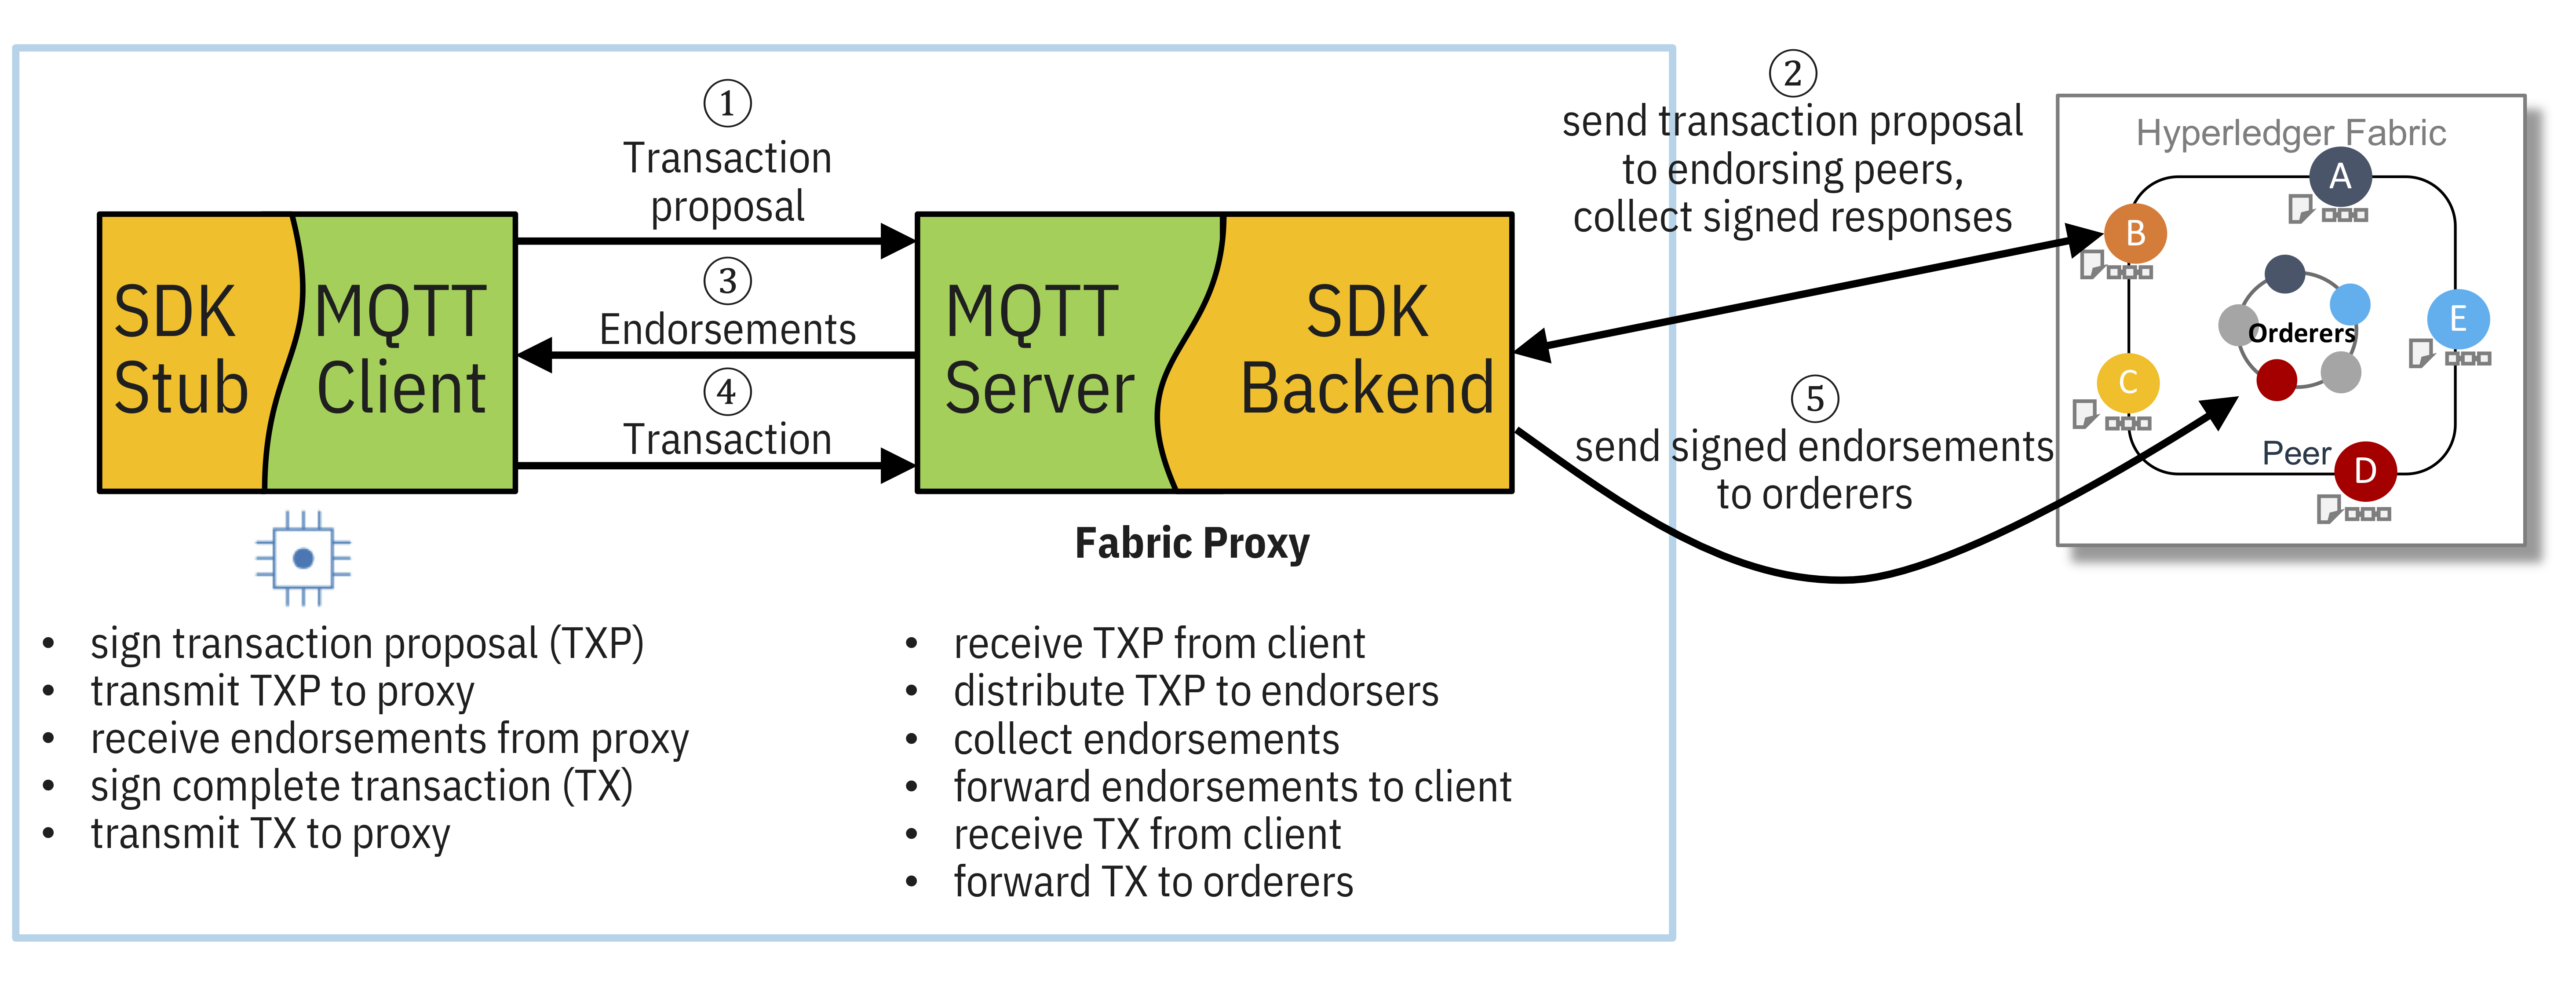
\includegraphics[width=1\textwidth]{images/6_performance/FabricSDKProxy_IBM.png}
    \caption{Proxy-SDK architecture \cite{proxy-sdk}}
    \label{fig:proxy-sdk}
\end{figure}
\section{Setup and Tools}
In this section we present the setup for the proof of concept as well as tools used for the performance analysis. 
\subsection{Proof of Concept}
As we presented in our case study in \ref{subsec:cold-chain-monitoring},
the Proxy SDK is used in a blockchain prototype solution for tracking, tracing and cold chain monitoring of pharmaceutical products that was developed by IBM Research Zürich. Particularly, sensors measure the temperature of containers that carry medicine and pharmaceutical products. Transactions of temperature and humidity sensor data are carried out by a Raspberry Pi which serves as a development platform for small-scale IoT devices. Transactions are sent to an \acrshort{mqtt} broker and the proxy listens to the relevant topics from the broker. The Fabric network consists of several peers (actors in the supply chain network) with a simplified single orderer scheme, running solo. 

We continue with a demonstration of the application. In \ref{fig:client-init}, the client gets authenticated, subscribes-publishes to the relevant topic and initiates a transaction. The proxy in \ref{fig:proxy-init}, gets authenticated, subscribes to the relevant topic and listens for incoming transactions. The transaction, initiated by the client, eventually arrives at the proxy.
In the meantime, proxy receives endorsement responses as seen in figure \ref{fig:proxy-mid} and the client receives them from proxy. Finally in figure \ref{fig:client-finalizing}, the client sends the final transaction to the proxy. The proxy \ref{fig:proxy-final} receives it and sends it to the network for ordering. 
\begin{figure}[H]
    \centering
    \includegraphics[width=0.9\textwidth]{images/6_performance/client.png}
    \caption{Client subscribes-publishes to a topic and initializes a transaction.}
    \label{fig:client-init}
\end{figure}

\begin{figure}[H]
    \centering
    \includegraphics[width=0.9\textwidth]{images/6_performance/cilient-finalizing.png}
    \caption{Client sends the final transaction.}
    \label{fig:client-finalizing}
\end{figure}

\begin{figure}[H]
    \centering
    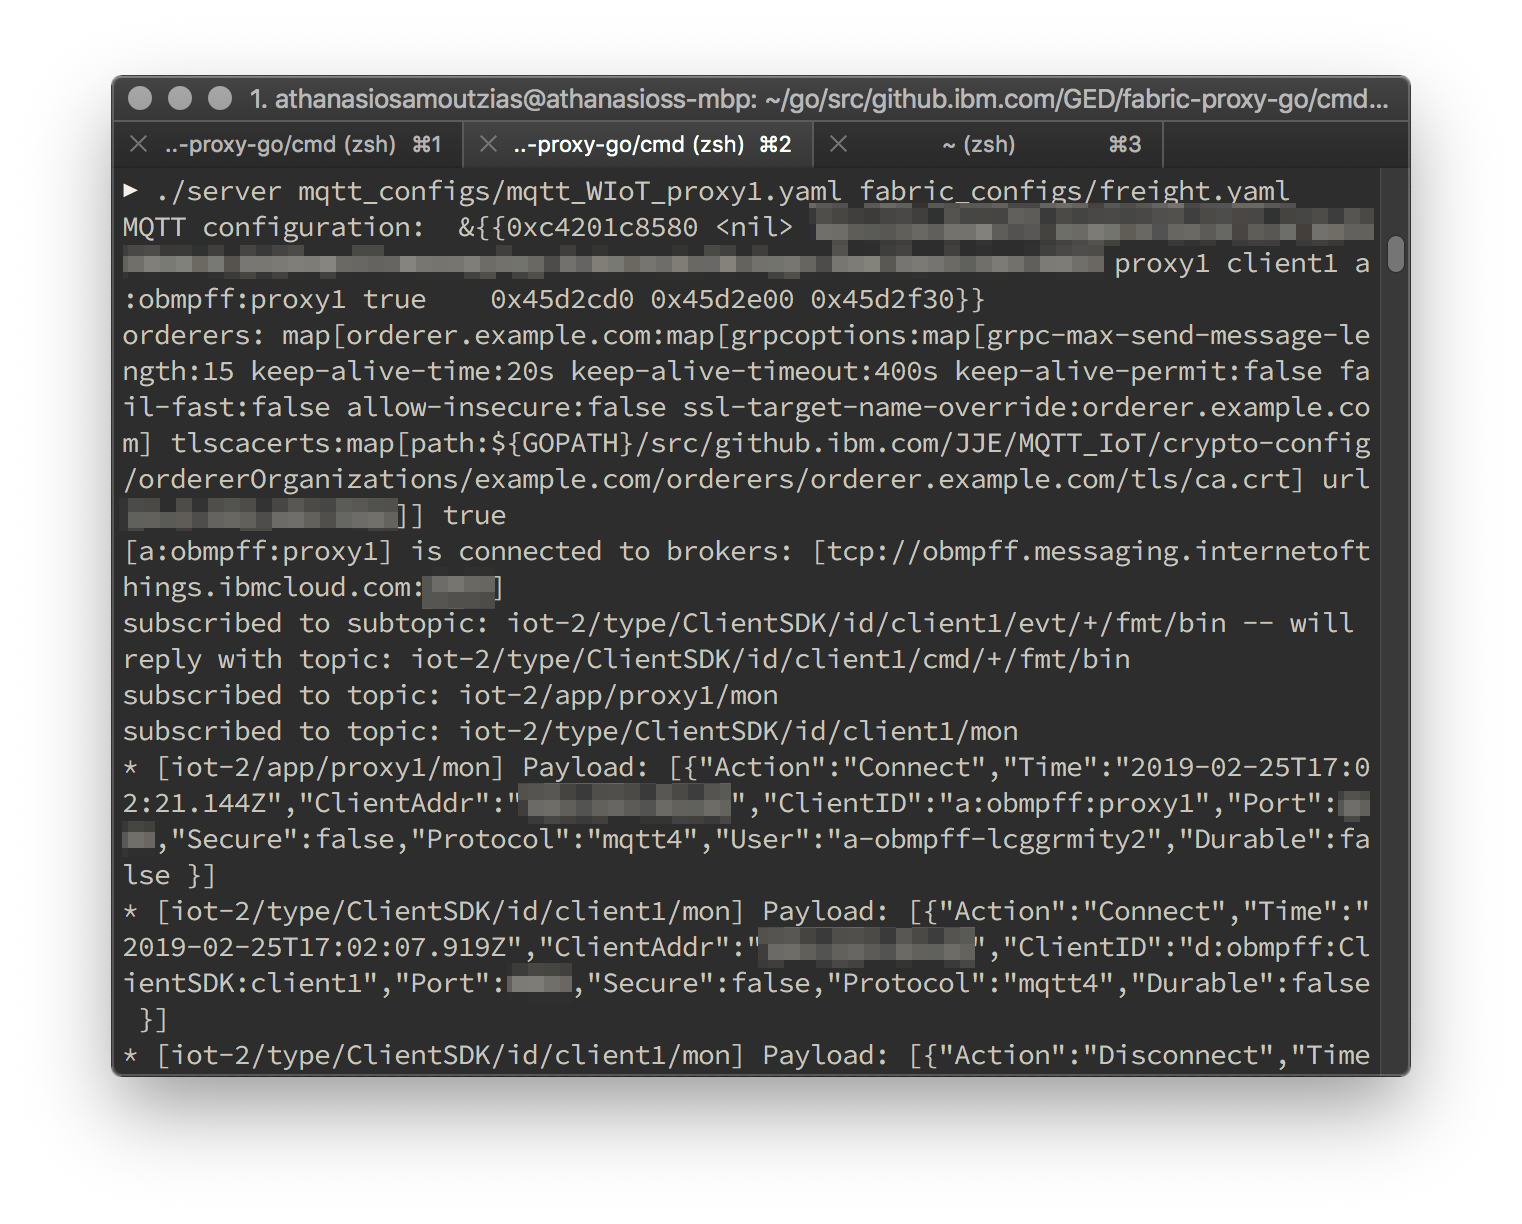
\includegraphics[width=0.9\textwidth]{images/6_performance/proxy-init.png}
    \caption{Proxy subscribes to topic and gets transaction from client.}
    \label{fig:proxy-init}
\end{figure}

\begin{figure}[H]
    \centering
    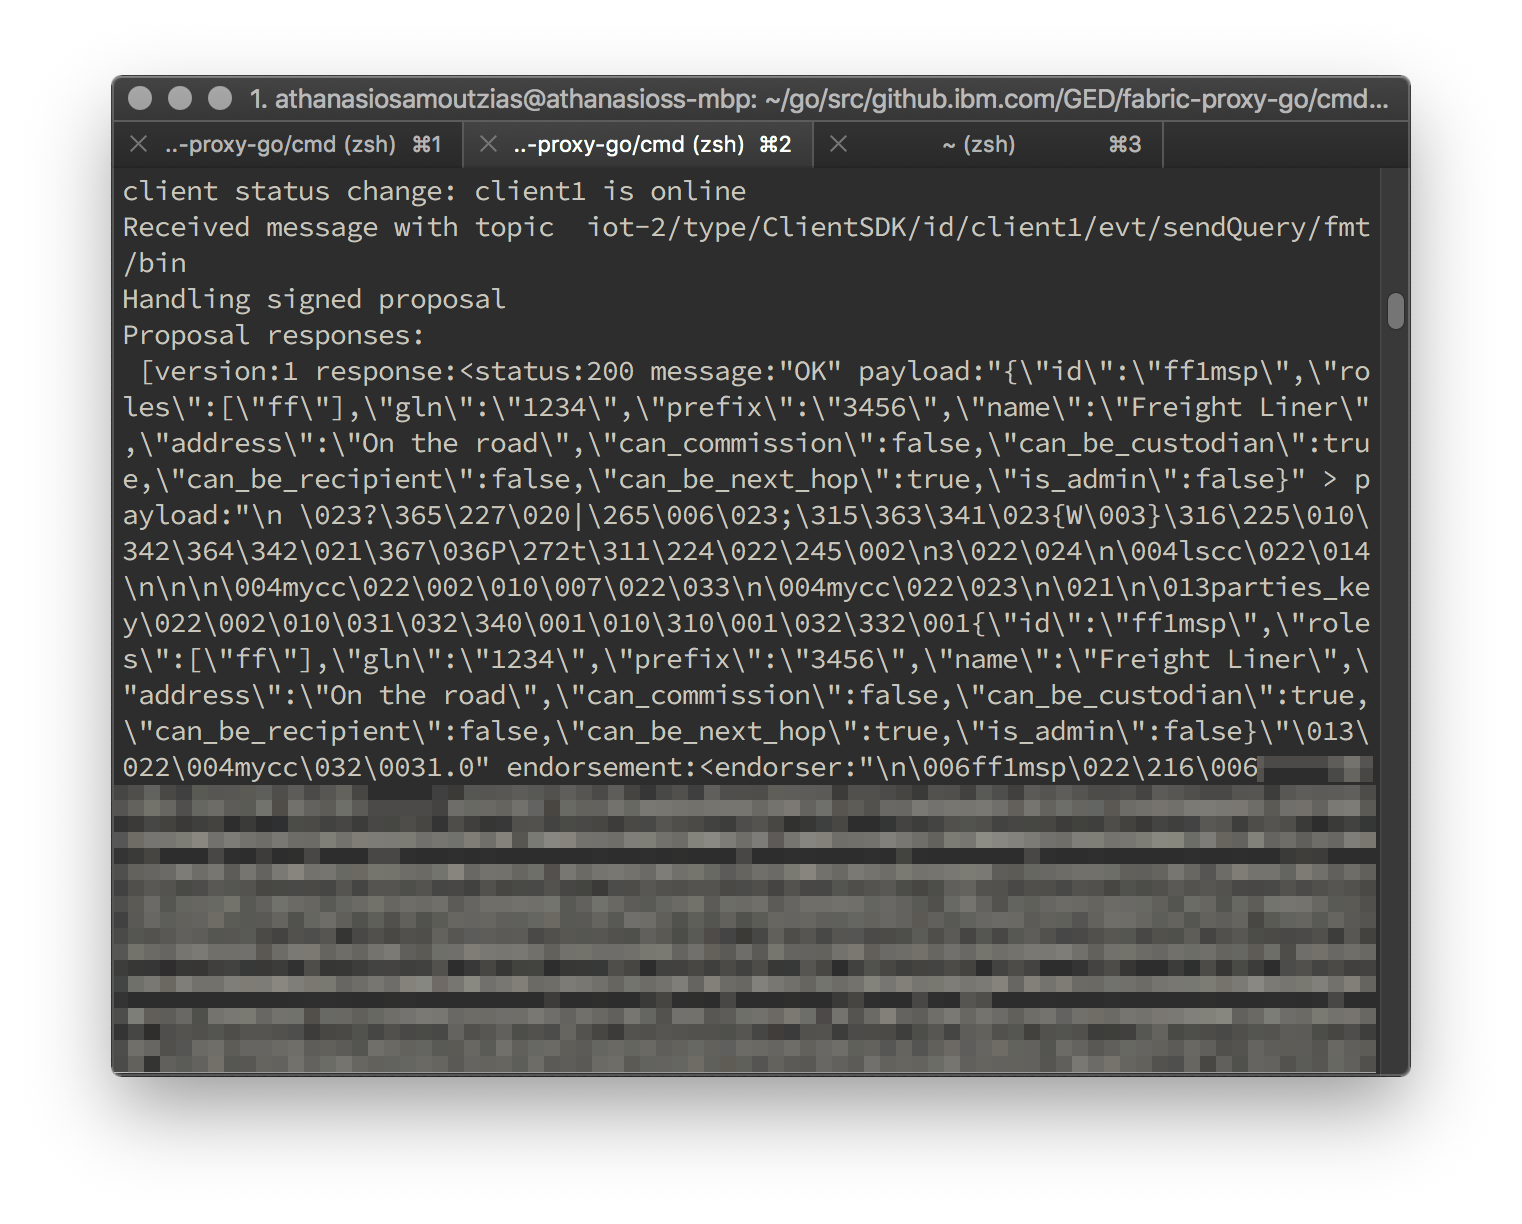
\includegraphics[width=0.9\textwidth]{images/6_performance/proxy-mid.png}
    \caption{Proxy gets responses from endorsers.}
    \label{fig:proxy-mid}
\end{figure}

\begin{figure}[H]
    \centering
    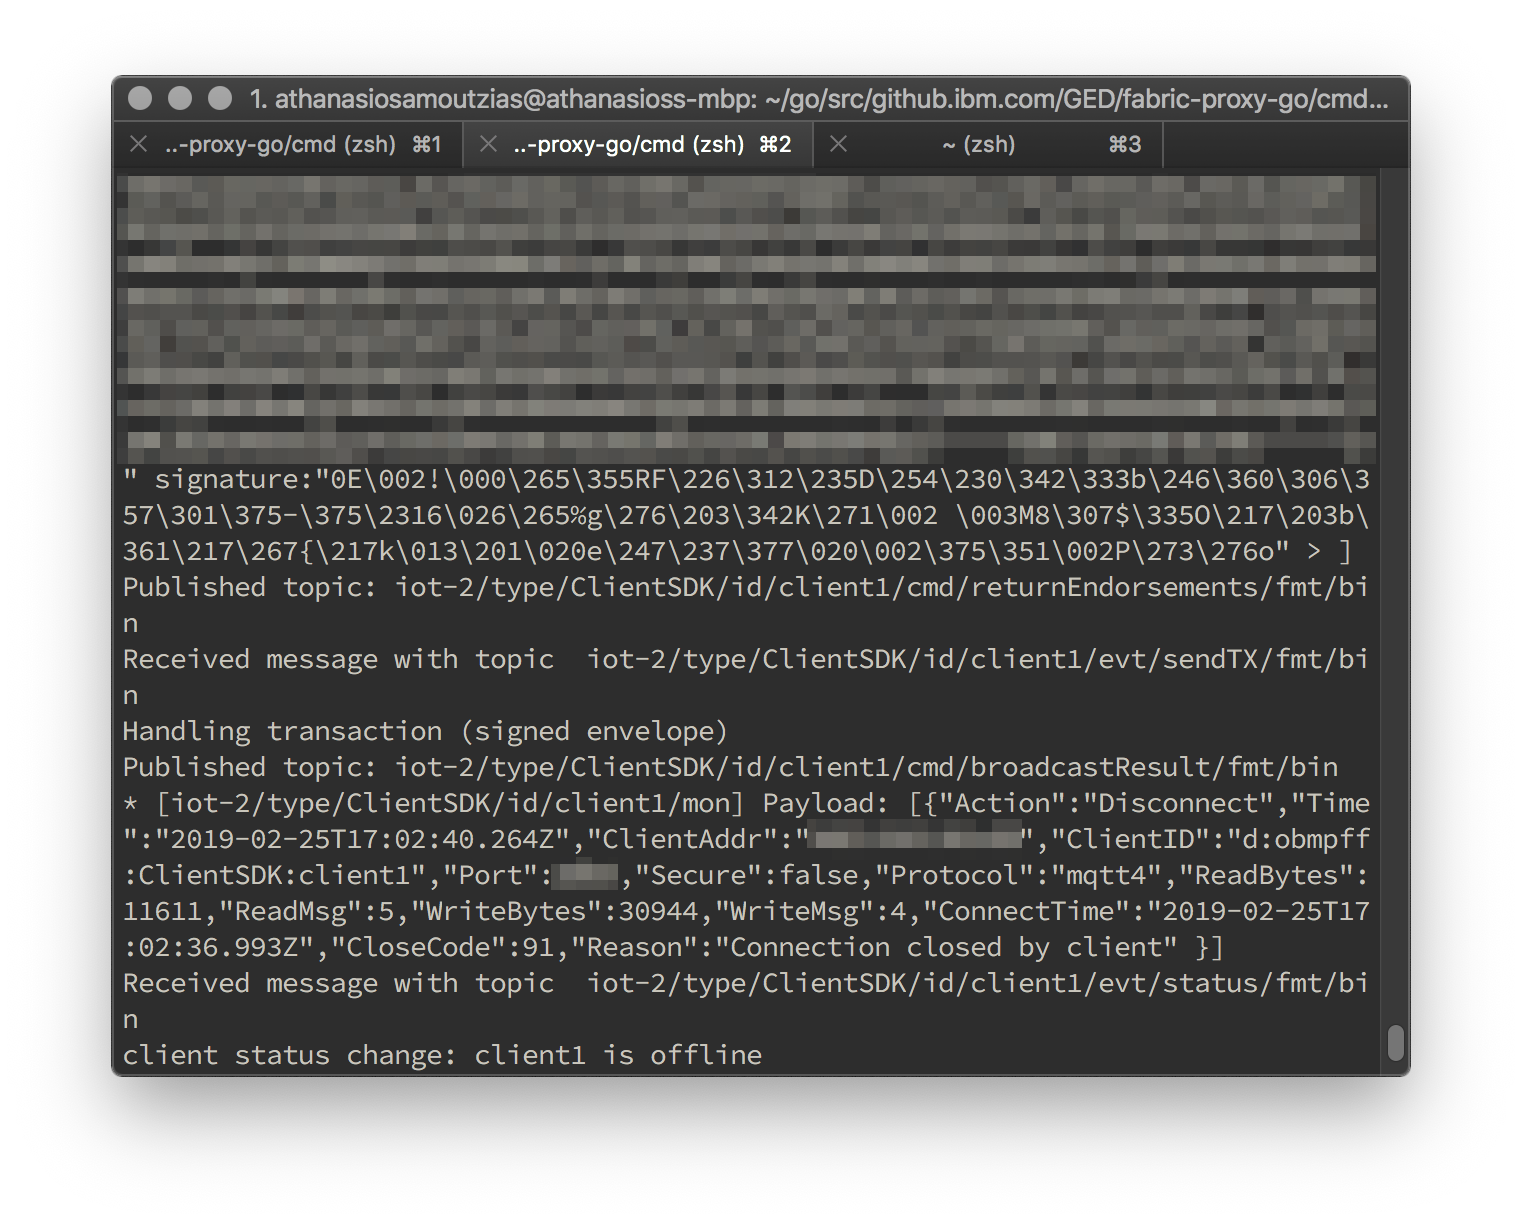
\includegraphics[width=0.9\textwidth]{images/6_performance/proxy-final.png}
    \caption{Proxy sends the final transaction to the Fabric network.}
    \label{fig:proxy-final}
\end{figure}

\subsection{Tools}
\subsubsection{Wireshark}
Wireshark is a packet analyser tool. It was used to troubleshoot the connection of the client to the proxy and Fabric network as well as check packet frequency and contents \cite{wireshark}.
\subsubsection{Activity monitor}
MacOS native activity monitor was used to cross reference results from Wireshark and profiling on network bandwidth and RAM usage \cite{instruments}.
\subsubsection{Golang}
Go is a language developed by Google and it's built with high performance networking and multiprocessing in mind \cite{golang}.
\subsubsection{pprof - Golang's profiling tool}
Profiling is a form of dynamic program analysis that measures the space complexity, the usage of particular instructions, frequency and duration of function calls and it serves as an aid to program optimization. Profiles can track heat-points of the program and help the user look for methods that can lead to improvements.
Google's Go language uses its own profiler called \verb|pprof|. It reads a collection of profiling samples in \verb|profile.proto| format and generates reports to visualize and help analyze the data. It can generate both text and graphical reports \cite{pprof}.
\subsubsection{Hardware used}
A Raspberry Pi used as a client and a laptop as a proxy. We should note here that Raspberry Pi does not offer cryptography acceleration hardware as modern fully fledged CPUs and that makes the cryptography algorithms slower and less efficient. \footnote{ARMv8, the architecture used in Raspberry Pi CPU, supports cryptography acceleration instructions but they are not implemented due to licensing costs.}
\begin{table}[h]
    \centering
    \begin{tabular}{c|c|c|c|c}
       Architecture  & Model & Cores/Threads & Frequency & Machine   \\
       \hline \hline
       x86  & Ιntel i7-4770HQ & 4/8 & 2.2GHz & Macbook Pro  \\
       ARMv8  & Broadcom BCM2837 & 4/4 & 1.2GHz & Raspberry Pi 3B \\
    \end{tabular}
    \caption{Hardware used for benchmarking and testing.}
    \label{tab:hardware-used}
\end{table}
\section{Performance findings}
In this section, we present our performance analysis results by first explaining the metrics used, then presenting the results and finally discussing them. The analysis was done with the lightweight client and results are from its perspective.

\subsection{Metrics}
\subsubsection{Times}
\begin{enumerate}
    \item \textbf{User}: Amount of time CPU spent in user space, outside the kernel, within the process. The time the process spends blocked does not count towards this metric. It represents only the actual CPU time used in executing the process.
    \item \textbf{System}: Amount of time CPU spent in the kernel space within the process. Mostly spent in system calls within the kernel, as opposed to library code, which is still running in user-space.
    \item \textbf{CPU}: Total processor time used by process since it started, calculated as $$cpu=user+system$$. We use it as an indicator to compare different binaries with a given CPU.
    \item \textbf{Wall}: Elapsed time of an executable, from start to finish.
    \item \textbf{Utilization}: Percentage of actual work done by the cpu during execution of the program defined as $$util=\frac{cpu}{wall}$$  
\end{enumerate}
\subsubsection{Call Graphs}
A control flow graph which represents calling relationships among functions in a program. Each node represents a procedure and each edge (f,g) indicates that procedure f calls g. A circle in the graph indicates recursive procedure calls. Profiler outputs dynamic call graphs that represent this execution of the program. Leaves account for the end functions that CPU spent most of its time.

\subsubsection{Methodology and Approach}
First, we start with CPU profiling. Inside the client's \verb|main()| function we add the CPU profiling snippet shown in figure \ref{fig:Profiling}. Our main focus on profiling is the call graph where we investigate heat-points and how much time each part of the program consumes. Then, without the profiling snippet, since profiling introduces an overhead, we use the commands \verb|time| to get our executable times. We continue with profiling the memory usage and get our call graphs. Again, with a fresh start, we capture packets and measure bandwidth usage. 
\begin{figure}[ht]
    \centering
    \lstinputlisting{code/profiling.go}
    \caption{Profiling method \cite{pprof}}
    \label{fig:Profiling}
\end{figure}
\subsection{CPU}
Go is built for concurrency, the program uses all cores during execution. We considered to emulate a one-core architecture with no cryptography acceleration to emulate a \acrfull{mcu} but it turned quite difficult and time consuming.

In table \ref{tab:CPU}, we see a notable decrease in CPU time from 130ms to 60ms making it a 53\% decrease in CPU resources. The wall time for each transaction is higher due to the network overhead, since we introduced two more intermediaries, the MQTT broker and proxy.
\begin{table}[H]
    \centering
    \begin{tabular}{||lllllll||}
    \hline
         SDK & on & user & sys & cpu & util & wall  \\
         \hline \hline
         Full & PC &70 & 60 & 130 & 7\% & 1.7s  \\
         \hline
         Lite & PC &40& 20 & 60 & 1\% & 3.1s\\
         \hline
         Lite & IoT &140& 30  & 170 & 2\% & 7s\\
         \hline
    \end{tabular}
    \caption{CPU times in milliseconds.}
    \label{tab:CPU}
\end{table}

Our conclusions from figure \ref{fig:cpu-prof-call} \footnote{Graph is zoom-able} are that cryptographical operations account of 28\% of the total executable usage, which is rather low considering that the Raspberry Pi does not have cryptography acceleration hardware. That means that cryptography operations are only a few and they introduce a small overhead. Accountable for the rest of the usage are data structures, memory operations and the MQTT service. The flow of the program is straight forward and we do not observe any unnecessary communication back and forth. 

We should note that profiling procedures that are fast and computationally inexpensive can be quite troublesome. One main reason is the resolution of the tool which is at 100Hz and we cannot easily observe leaks and inefficiencies that could accumulate over time.
\begin{figure}[h]
    \centering
    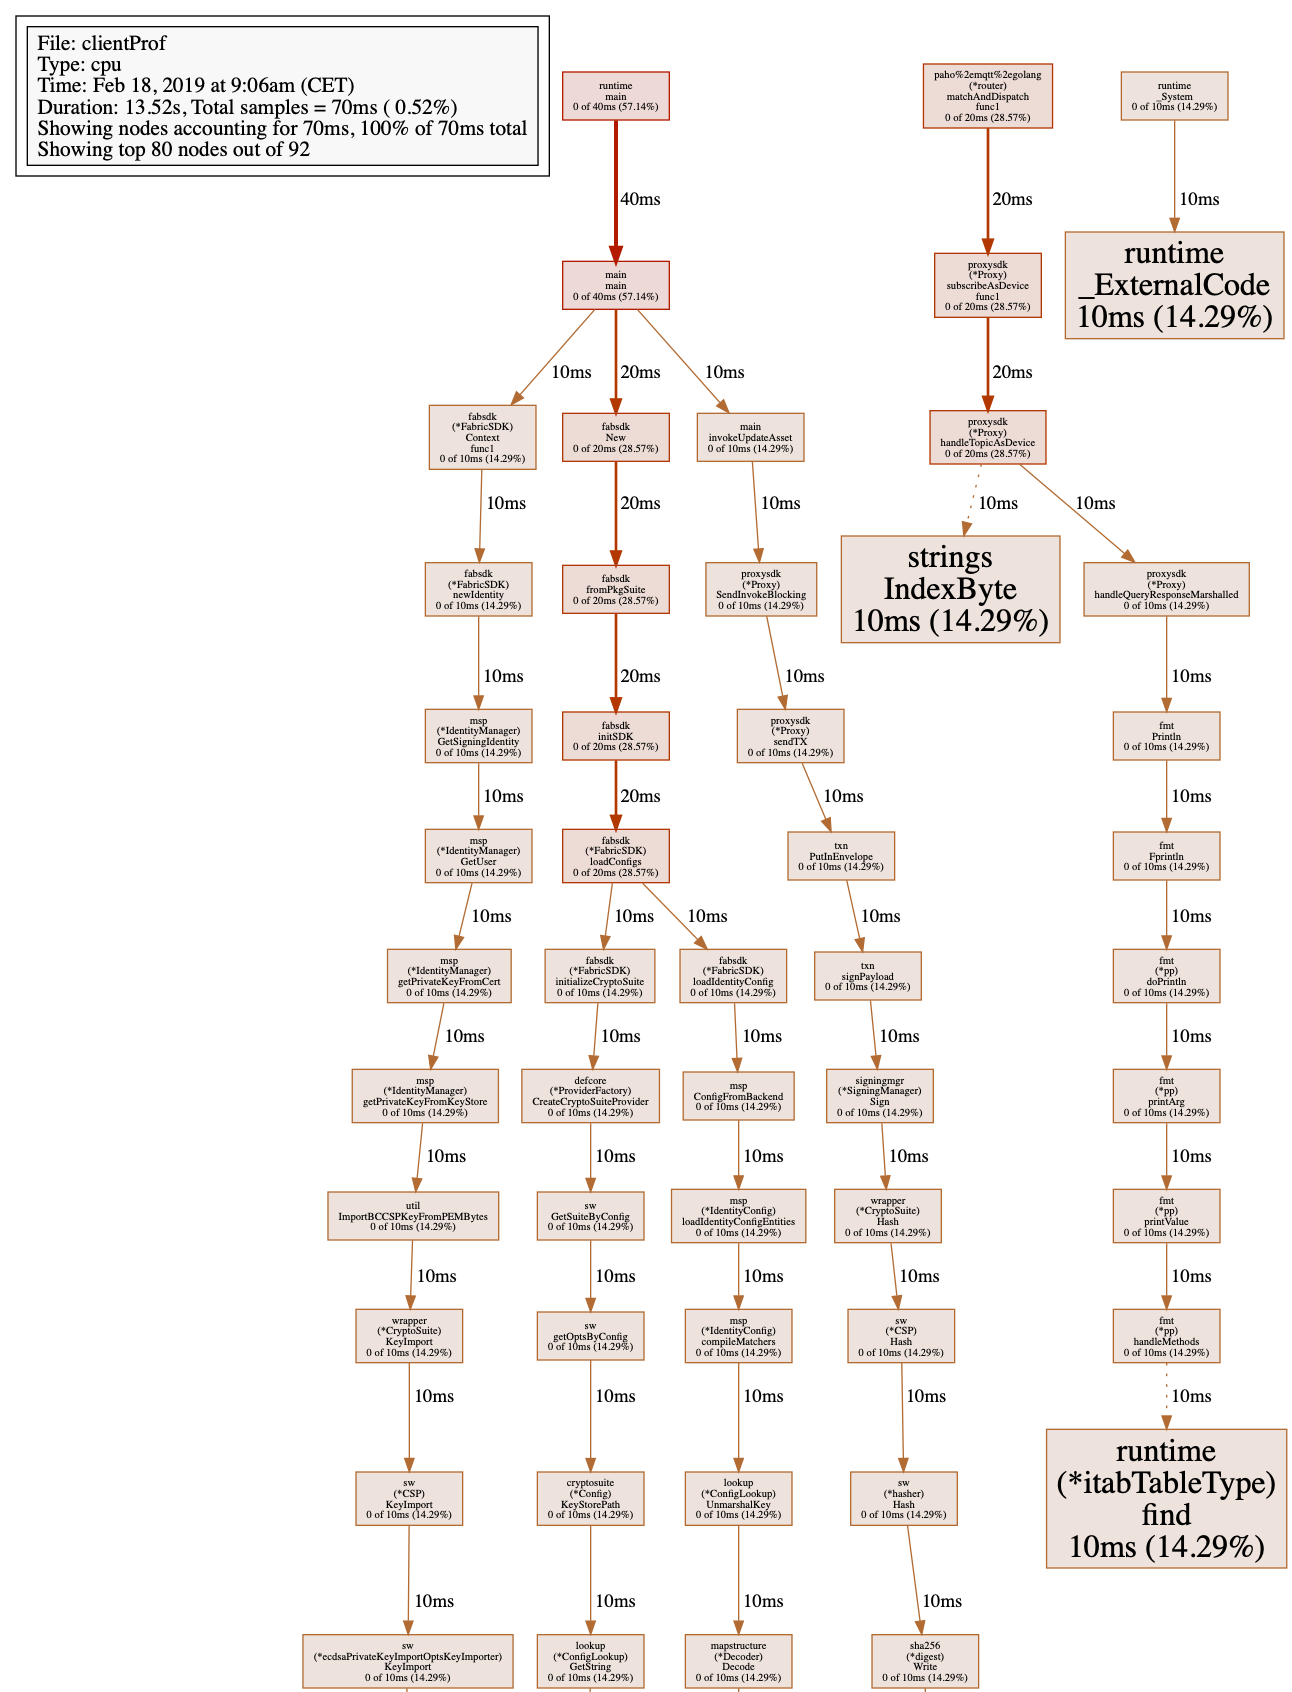
\includegraphics[width=1\textwidth]{images/6_performance/pi-cpu-call-top.png}
    \caption{Call-graph of client on Raspberry Pi, leaves represent where the CPU spent most of its time.}
    \label{fig:cpu-prof-call}
\end{figure}
\begin{figure}[h]
    \centering
    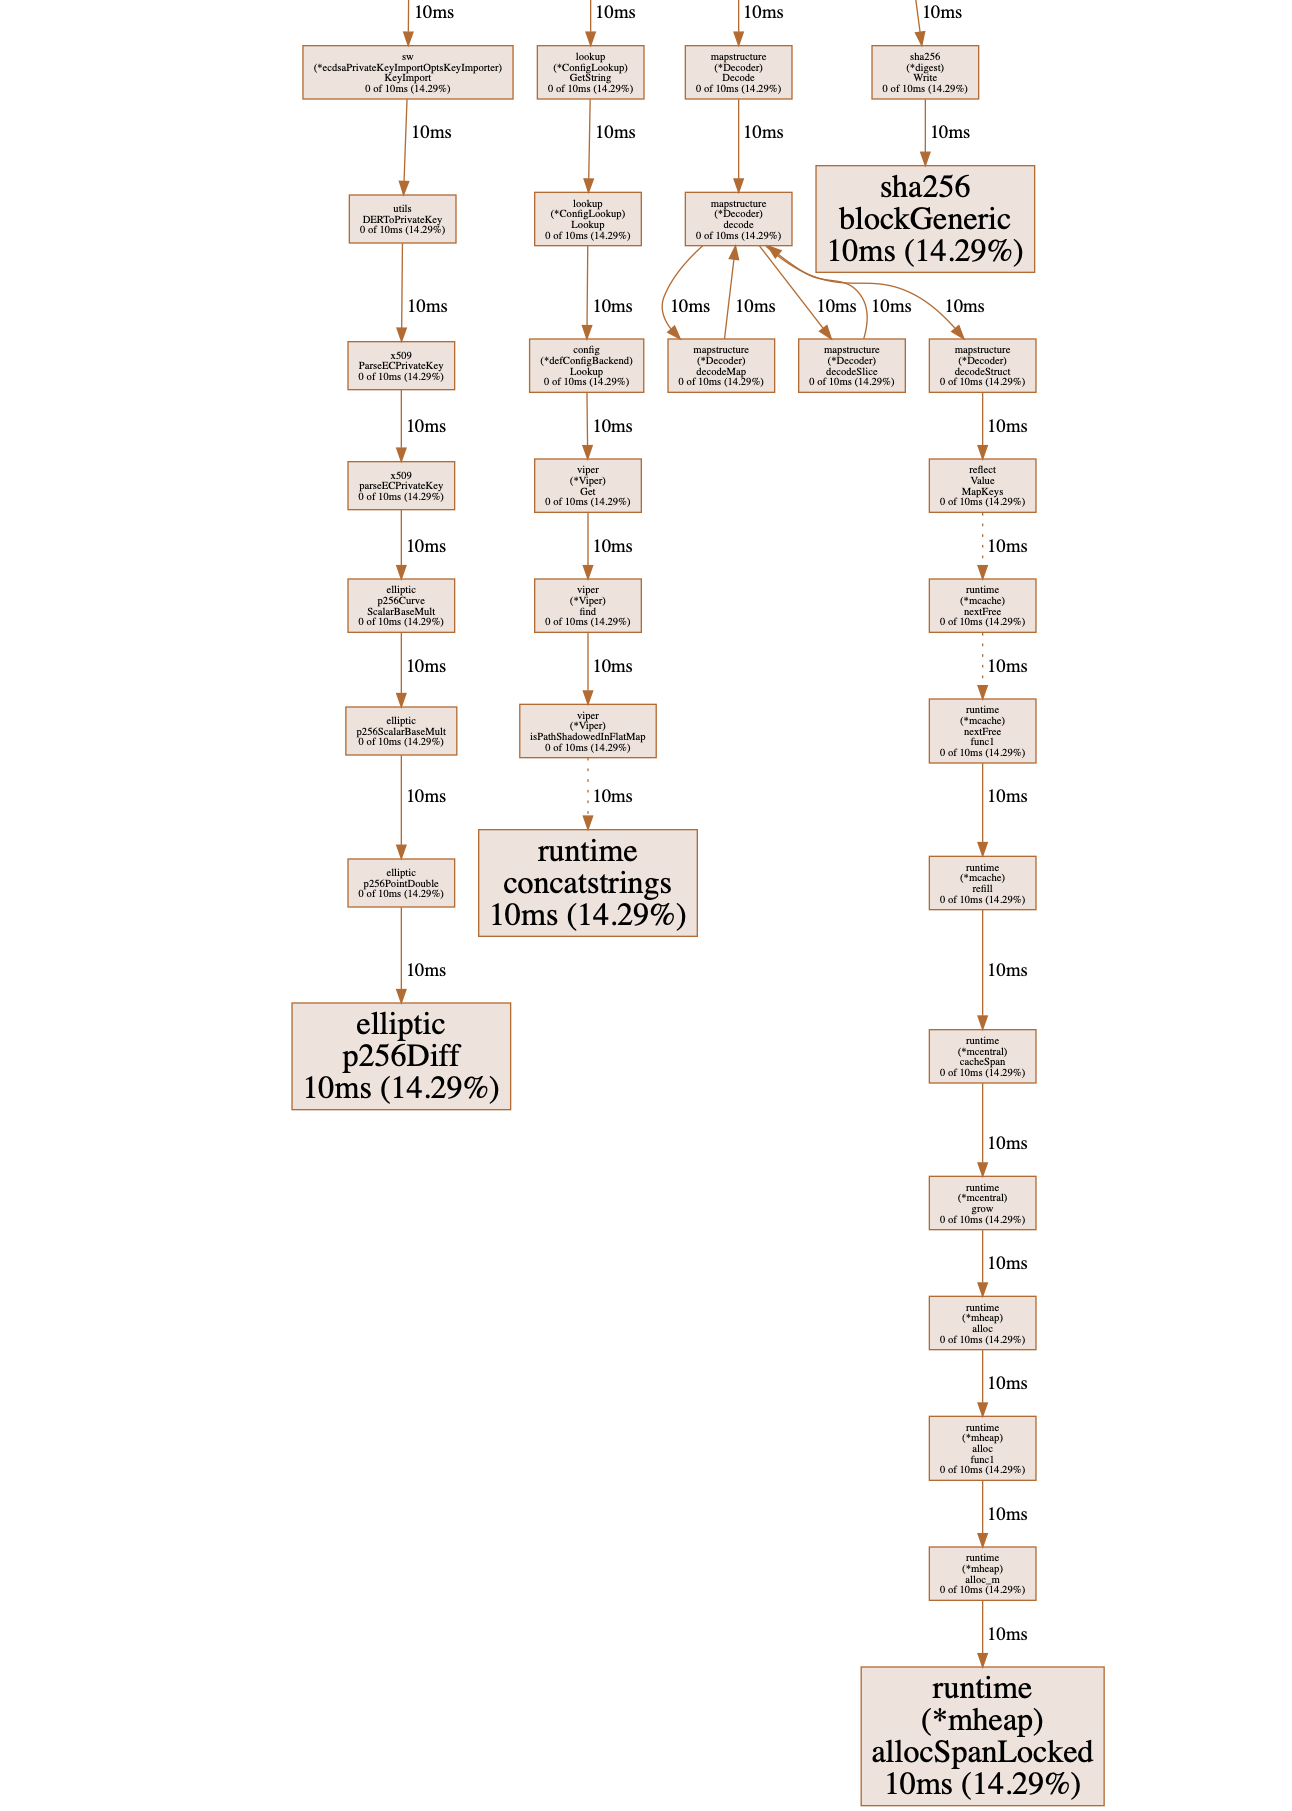
\includegraphics[width=1\textwidth]{images/6_performance/pi-cpu-call-bottom.png}
    \caption{Bottom part of call-graph.}
    \label{fig:cpu-prof-call-bottom}
\end{figure}

\subsection{Memory}
In table \ref{tab:RAM}, we observe that memory-wise both SDKs are at the same order, the executable size and the RAM they consume hardly differ.
\begin{table}[H]
    \centering
    \begin{tabular}{c|c|c}
        SDK &  RAM & Size\\
       Full  & 3.1  & 25.7\\
       Lite  & 3.5 & 27 \\
    \end{tabular}
    \caption{RAM consumed during execution and binary sizes, values in MB.}
    \label{tab:RAM}
\end{table}
\subsection{Bandwidth and Latency}
In table \ref{tab:Bandwidth}, we see a notable decrease in network usage. Specifically, a 21\% decrease in packets sent and a 81\% decrease in packets received making it a 71\% overall improvement. Since every \verb|KB| in remote set-ups cost, a 71\% reduced bandwidth is quite significant.
\begin{table}[H]
    \centering
    \begin{tabular}{c|c|c|c|c}
        SDK & Sent & Rcvd & Sent Packets & Rcvd Packets  \\
        Full & 14KB & 90KB & 47 & 112 \\
        Lite & 11KB & 17KB & 28 & 31 \\

    \end{tabular}
    \caption{Bandwidth consumed for one transaction.}
    \label{tab:Bandwidth}
\end{table}